

\documentclass[10pt, twocolumn, twoside]{article}
%List of article class defaults (with some useful options in brackets) = A4, 10pt [11pt, 12pt], onecolumn [twocolumn], oneside [twoside], notitlepage, portrait, equations-centre-rightlabel, final [draft]. 
\usepackage{amsmath}
\usepackage[left=0.70cm, right=0.70cm, top=0.70cm, bottom=0.70cm]{geometry} % sort out the too large LaTeX default margins.
\usepackage{graphicx} %for importing graphics, see \begin{figure} below.
\usepackage{amssymb,amsmath} % add some standard packages for maths and symbols
\usepackage[colorlinks=true,linkcolor=blue]{hyperref} % turns all latex references into hyperlinks, useful if you have e.g. a large document with a large table of contents. Note that a known Apple bug is that the hyperlinks exist in the pdf, but don't they show up under the Apple pdf reader, Preview. Try Adobe Reader for your pdf on a Mac.

\usepackage{lipsum} % for generating dummy text, you can delete all lipsum commands in your final document, including this one.

\author{E. Davies\\PH1999 report}

\title{Dark Matter Project}

\date{\today}

%everything before this line is called the 'preamble'. Now we begin the document. 

\begin{document}

\maketitle %this uses the author, title, date information given in the preamble to make a title.

\begin{git}
https://github.com/Emlyn25/Physics-project-code-and-images
\end{git}

%The basic structure of LaTeX is that of \beginning an {environment}, and ending it. Above is the 'abstract' environment. Note the figure, table and equation environments below. 



\begin{itemize}
  \item M=first mass(kg)
  \item m=second mass(kg)
  \item v=velocity(m/s)
  \item r=radius(m)
  \item F=Force(N)
  \item a=acceleration(m/s^2)
  
  \item G=Gravitational constant(6.67x10^-11)
\end{itemize}


\section{Weak 1}
The relationship between acceleration, velocity and radius in uniform circular motion is:
\label{GaussE}
\begin{equation}
a=v^2/r
\end{equation}
The gravitational force between two point masses is:
%an example displayed equation
\begin{equation}
\label{GaussE}
F=GMm/r^2
\end{equation}
from these you can calculate the equation for velocity as a function of mass and radius:

\begin{equation*}
\label{GaussE}
\begin{aligned}
F=GMm/r^2 ----F=ma ----a=v^2/r
\end{aligned}
\end{equation*}
\begin{equation*}
\label{GaussE}
\begin{aligned}
F=mv^2/r
\end{aligned}
\end{equation*}
\begin{equation*}
\label{GaussE}
\begin{aligned}
GMm/r^2=mv^2/r
\end{aligned}
\end{equation*}
\begin{equation*}
\label{GaussE}
\begin{aligned}
GM/r^2=v^2/r
\end{aligned}
\end{equation*}
\begin{equation*}
\label{GaussE}
\begin{aligned}
GM/r=v^2
\end{aligned}
\end{equation*}
\begin{equation*}
\label{GaussE}
\begin{aligned}
\sqrt(GM/r)=v
\end{aligned}
\end{equation*}
Given this you can calculate the mass within a sphere, when talking about galaxy's,
this is visualised as a gas cloud with density ρ and the mass is the all the "particles"
within the radius this is called Mc(r) for contained mass within the radius.
v=Volume(kg/m^3) V=Velocity(m/s):

\begin{equation*}
\label{GaussE}
\begin{aligned}
\rho= m/v----v=4/3\pi r^3---\sqrt(GM/r)=V
\end{aligned}
\end{equation*}
\begin{equation*}
\label{GaussE}
\begin{aligned}
 m=\rho v
\end{aligned}
\end{equation*}
\begin{equation*}
\label{GaussE}
\begin{aligned}
 m= 4/3\pi r^3\rho
\end{aligned}
\end{equation*}
\begin{equation*}
\label{GaussE}
\begin{aligned}
\sqrt(4/3\pi r^3\rho G/r)=V
\end{aligned}
\end{equation*}
\begin{equation*}
\label{GaussE}
\begin{aligned}
\sqrt(4/3\pi r^2\rho G)=V
\end{aligned}
\end{equation*}
\begin{equation*}
\label{GaussE}
\begin{aligned}
r\sqrt(4/3\pi \rho G)=V
\end{aligned}
\end{equation*}
the velocity is now positively directly proportion to the radius
this means you can predict a velocity based on the radius of a galaxy.
\begin{figure}[ht] .
\includegraphics[width=\columnwidth]{capture.png}
\caption[width=\columnwidth]{BLUE = Predicted data using mass of galaxy \\
ORANGE = Actual velocity and radius data of galaxy} \\
This shows us that the predicted velocity based on the mass does not match the velocity observed (all other variables are the same). Is the equation wrong?! No, The Universal law of gravitation is well, universal, and proven. So that leaves a very odd conclusion, that somehow within the galaxy there is more mass that we cannot see or interact with but still has a gravitational effect changing the velocity as there is actually more mass there.
\end{figure}




\section{Weak2}
This equation gives you just the mass of the dark matter based on the radius:
\begin{equation*}
\label{GaussE}
\begin{aligned}
M_c^D^M= 4\pi\rho_0r_c^2(r-r_c \arctan{r/r_c})
\end{aligned}
\end{equation*}
This allows scientists to plot the theoretical amount of dark matter on a Velocity, Radius graph along with the actual data, and the original prediction based on visible mass. and the dark matter curve, then the Dark matter and visible matter can be added together, this is should closely resemble the actual data as its all types of matter visible and dark.
\pagebreak



\begin{figure}[ht] .
\includegraphics[width=\columnwidth]{captureWEAK2.png}
\caption[width=\columnwidth]{RED = Actual Velocity and radius measured \\
ORANGE = original prediction of velocity based on visible mass} \\
GREEN = Dark matter curve, the velocity based on the dark matter alone \\
BLUE = Dark and Visible matter added together to give the final velocity \\
As you can see the original prediction based on actual mass and dark matter mass don't get the same velocity
as the actual data. However when you add these together, so both dark and visible matter in a galaxy, it closely
resembles the actual data of velocity and radius. This seemingly Validates the dark matter theory.

\end{figure}

\section{Weak3}
This equations will allow you to find a line of best fit from a set of points The best line is defined by X^2:

\begin{equation*}
\label{GaussE}
\begin{aligned}
X^2=\sum_{i}^{}[(y_i-f(x_i))^2/\sigma_i^2]
\end{aligned}
\end{equation*}

\begin{figure}[ht] .
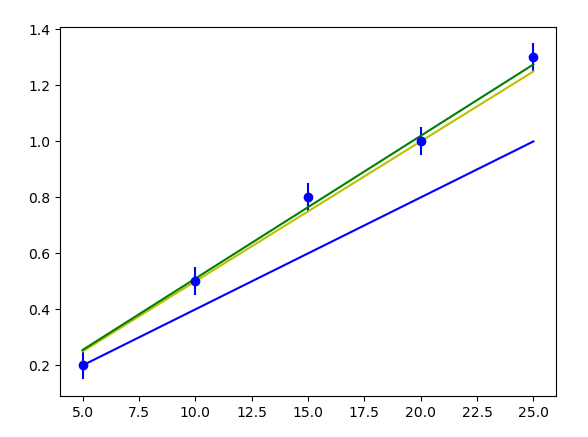
\includegraphics[width=\columnwidth]{CaptureWEAK3.PNG}
\caption[width=\columnwidth]{DARK GREEN = Line of best fit \\
LIGHT GREEN-YELLOW = manually entered 0.05x for comparison} \\
BLUE = Original starting point for reference \\
At the start the blue line was already visible, this is a good visual aid as you know its 0.04x, from this you can make an educated guess that the line of best fit connecting the blue dots with error capacitance wither side in the y-axis, is about 0.05x. The code that calculates this takes the standard deviation from the points the error margin and both x and y. The line that it calculates is dark green and it goes right through the points. The yellow line is a manually entered 0.05x line. As you can see it is very close to the calculated line meaning that the line of best fit is in fact ~0.05x
\end{figure}

\begin{figure}[ht] .
\includegraphics[width=\columnwidth]{captureQ16.png}
\caption[width=\columnwidth]{PURPLE = Actual Velocity and radius measured \\
LIGHT GREEN = original prediction of velocity based on visible mass} \\
RED = Dark matter curve, the velocity based on the dark matter alone \\
ORANGE = Dark and Visible matter added together to give the final velocity \\
BLUE= experimental p_0 optimisation that takes into account X^2 and minimises it to give to make a new line of best fit for many different p_0 that give a more accurate mass picture(with 0.05 Y-error bounds)
As you can see its very similar to the velocity from the mass given. I will admit i got quite stuck at this point as the question was quite difficult to understand exactly what i am meant to code!
\end{figure}
\begin{thebibliography}{1}



\end{thebibliography}
for unknown reasons new text typed normally on this doc will not display correctly and will go off the page The git hib will have the .tex file on it to see more!


\end{document}
